% v1 vs v2 confirmation interface (appendix figure). Compile: xelatex interface.tex
\documentclass[border=1pt]{standalone}
\usepackage{fontspec}
\setmainfont{OpenSans}[Path=../../fonts/,Extension=.ttf,UprightFont=*-Regular,BoldFont=*-Bold,
  ItalicFont=*-Italic,BoldItalicFont=*-BoldItalic]
\usepackage{tikz}
\usetikzlibrary{arrows.meta,positioning}
\definecolor{trust}{HTML}{0072B2}
\definecolor{ink}{HTML}{222222}
\definecolor{bad}{HTML}{D55E00}
\begin{document}\hyphenpenalty=10000\exhyphenpenalty=10000
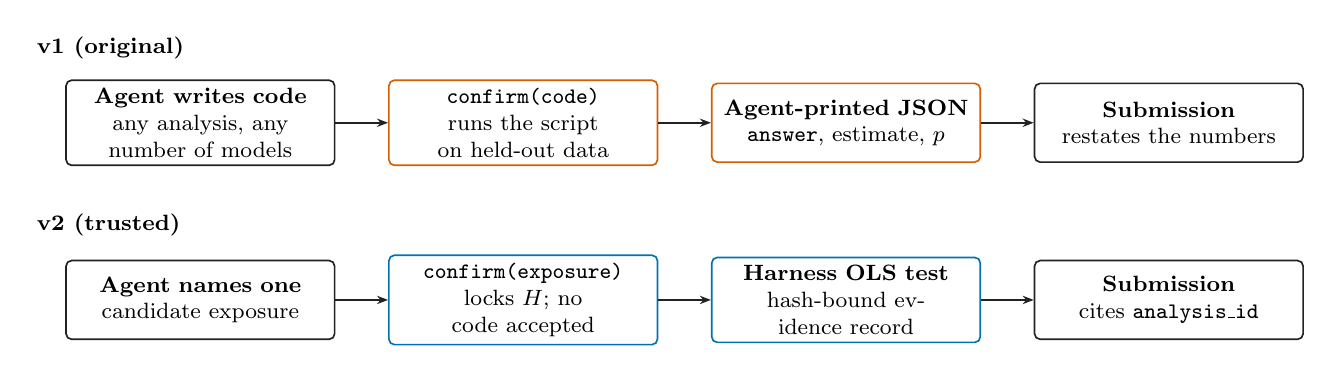
\begin{tikzpicture}[font=\fontsize{8}{9.6}\selectfont, >={Stealth[length=4pt]},
  b/.style={draw=#1, rounded corners=2pt, line width=0.6pt, align=center, minimum height=1.0cm,
            text width=3.2cm, inner sep=3pt, fill=white},
  a/.style={->, line width=0.7pt, draw=ink}]
\node[anchor=west, font=\fontsize{8.5}{10}\selectfont\bfseries] at (-0.2, 1.25) {v1 (original)};
\node[b=ink]  (v1a) at (2.0, 0.3) {\textbf{Agent writes code}\\ any analysis, any number of models};
\node[b=bad]  (v1b) at (6.1, 0.3) {\textbf{\texttt{confirm(code)}}\\ runs the script on held-out data};
\node[b=bad]  (v1c) at (10.2, 0.3) {\textbf{Agent-printed JSON}\\ \texttt{answer}, estimate, $p$};
\node[b=ink]  (v1d) at (14.3, 0.3) {\textbf{Submission}\\ restates the numbers};
\draw[a] (v1a) -- (v1b); \draw[a] (v1b) -- (v1c); \draw[a] (v1c) -- (v1d);
\node[anchor=west, font=\fontsize{8.5}{10}\selectfont\bfseries] at (-0.2, -1.0) {v2 (trusted)};
\node[b=ink]   (v2a) at (2.0, -1.95) {\textbf{Agent names one}\\ candidate exposure};
\node[b=trust] (v2b) at (6.1, -1.95) {\textbf{\texttt{confirm(exposure)}}\\ locks $H$; no code accepted};
\node[b=trust] (v2c) at (10.2, -1.95) {\textbf{Harness OLS test}\\ hash-bound evidence record};
\node[b=ink]   (v2d) at (14.3, -1.95) {\textbf{Submission}\\ cites \texttt{analysis\_id}};
\draw[a] (v2a) -- (v2b); \draw[a] (v2b) -- (v2c); \draw[a] (v2c) -- (v2d);
\end{tikzpicture}
\end{document}
